%\documentclass[c]{beamer}  % [t], [c], или [b] --- вертикальное выравнивание на слайдах (верх, центр, низ)
%\documentclass[handout]{beamer} % Раздаточный материал (на слайдах всё сразу)


\documentclass[9pt,pdf]{beamer} % Соотношение сторон
\usepackage[labelfont=bf]{caption}
\usepackage{subfig} % for subfigures
\usepackage{bm}
%\usetheme{Bergen}
\usetheme{Berlin}
%\setbeamertemplate{footline}[frame number]
%\usetheme{Warsaw}
\beamertemplatenavigationsymbolsempty
%\useoutertheme{тема}
%\useinnertheme{тема} 

\setbeamercolor{background canvas}{bg=white}
\useinnertheme[shadow]{rounded}

%%% Работа с русским языком
\usepackage{cmap}					% поиск в PDF
\usepackage{mathtext} 				% русские буквы в формулах
\usepackage[T2A]{fontenc}			% кодировка
\usepackage[utf8]{inputenc}			% кодировка исходного текста
\usepackage[english,russian]{babel}	% локализация и переносы
\usepackage{graphicx}
\usepackage{geometry}
\usepackage{lipsum}
%% Beamer по-русски
\newtheorem{rtheorem}{Теорема}
\newtheorem{rproof}{Доказательство}
\newtheorem{rexample}{Пример}

%%% Дополнительная работа с математикой
\usepackage{amsmath,amsfonts,amssymb,amsthm,mathtools} % AMS
\usepackage{icomma} % "Умная" запятая: $0,2$ --- число, $0, 2$ --- перечисление

%% Номера формул
%\mathtoolsset{showonlyrefs=true} % Показывать номера только у тех формул, на которые есть \eqref{} в тексте.
%\usepackage{leqno} % Нумерация формул слева
\usepackage{bm}
%% Свои команды
\DeclareMathOperator{\sgn}{\mathop{sgn}}
\newcommand{\myfigref}[2]{~\ref{#1}.\subref{#2}}% <---- a new macro for referring to a subfigure
% \myfigref{label: fig}{label: subfig}
\newcommand{\T}{^{\mathsf{T}}}
\DeclareMathOperator*{\argmax}{arg\,max}  % in your preamble
\DeclareMathOperator*{\argmin}{arg\,min}  % in your preamble 

%%% Работа с картинками
\usepackage{graphicx}  % Для вставки рисунков
\setlength\fboxsep{3pt} % Отступ рамки \fbox{} от рисунка
\setlength\fboxrule{1pt} % Толщина линий рамки \fbox{}
\usepackage{wrapfig} % Обтекание рисунков текстом

%%% Работа с таблицами
\usepackage{array,tabularx,tabulary,booktabs} % Дополнительная работа с таблицами
\usepackage{longtable}  % Длинные таблицы
\usepackage{multirow} % Слияние строк в таблице
\usepackage[labelfont=bf]{caption}
%%% Программирование
\usepackage{etoolbox} % логические операторы

%%% Другие пакеты
\usepackage{lastpage} % Узнать, сколько всего страниц в документе.
\usepackage{soul} % Модификаторы начертания
\usepackage{csquotes} % Еще инструменты для ссылок
%\usepackage[style=authoryear,maxcitenames=2,backend=biber,sorting=nty]{biblatex}
\usepackage{multicol} % Несколько колонок

%%% Картинки
\usepackage{tikz} % Работа с графикой
\usepackage{pgfplots}
\usepackage{pgfplotstable}

\title{Пространственно-временные характеристики в задаче декодирования временных рядов.}
\author{Дорин Даниил Дмитриевич}
\date{\today}
\institute[Московский физико-технический институт]{Московский физико-технический институт }

\setbeamercovered{transparent = 15}

\begin{document}

	\begin{frame}{}
		\maketitle
	\end{frame}
%%%%%%%%%%%%%%%%%%%%%%%%%%%%%%%%%%%%%%%%%%%%%%%%%%%%%%%%%%%%%%%%%%%%%%%%%%%%%%%%%%%%%%%%%%%%%%%%%%%%%%%%%%%%%%%%%%%%%%%%%%%%%%%%%%%%%%%%%%%%%%

%%%%%%%%%%%%%%%%%%%%%%%%%%%%%%%%%%%%%%%%%%%%%%%%%%%%%%%%%%%%%%%%%%%%%%%%%%%%%%%%%%%%%%%%%%%%%%%%%%%%%%%%%%%%%%%%%%%%%%%%%%%%%%%%%%%%%%%%%%%%%%
\begin{frame}{Цель работы}
    \begin{block}{Исследуются}
        Пространственно-временные характеристики в задаче декодирования временных рядов. Основной целью анализа сигнала в данном исследовании является классификация электроэнцефалограммы (ЭЭГ).
    \end{block}
    
    \begin{block}{Требуется}
        Предложить метод классификации сигнала, основанный на анализе пространственно-временных характеристик между временными рядами, полученными при регестрации сигнала несколькими датчиками.
    \end{block}
    \begin{block}{Основное предположение}
    \begin{itemize}
        \item Зависимость между временными рядами значима в задаче декодирования и ее можно учитывать, переходя в касательное пространство с помощью Римановой геометрии.
    \end{itemize}
    \end{block}
\end{frame}

%%%%%%%%%%%%%%%%%%%%%%%%%%%%%%%%%%%%%%%%%%%%%%%%%%%%%%%%%%%%%%%%%%%%%%%%%%%%%%%%%%%%%%%%%%%%%%%%%%%%%%%%%%%%%%%%%%%%%%%%%%%%%%%%%%%%%%%%%%%%%%
\begin{frame}{Постановка задачи}
    Исследуется задача декодирования временного ряда. Пусть имеется некоторый непрерывный процесс (активность головного мозга):
$$\mathcal{V}(\tau),~\tau \in \mathbb{R}$$
Тогда данные выборки ~--- это регистрируемый сигнал, то есть реализация процесса $\mathcal{V}(\tau)$:
$$\bm{X} = \left[\bm{x}_1,\dots, \bm{x}_{T}\right],~\bm{x}_t \in \mathbb{R}^K
$$
Здесь $K$ ~--- число каналов. $T$ ~--- число измерений сигнала с частотой $\mu$ за время $\tau$:
$$T = \tau \mu$$
$$\bm{x}_{\tau \mu} \approx \mathcal{V}(\tau)$$
\end{frame}
%%%%%%%%%%%%%%%%%%%%%%%%%%%%%%%%%%%%%%%%%%%%%%%%%%%%%%%%%%%%%%%%%%%%%%%%%%%%%%%%%%%%%%%%%%%%%%%%%%%%%%%%%%%%%%%%%%%%%%%%%%%%%%%%%%%%%%%%%%%%%%


%%%%%%%%%%%%%%%%%%%%%%%%%%%%%%%%%%%%%%%%%%%%%%%%%%%%%%%%%%%%%%%%%%%%%%%%%%%%%%%%%%%%%%%%%%%%%%%%%%%%%%%%%%%%%%%%%%%%%%%%%%%%%%%%%%%%%%%%%%%%%%
\begin{frame}{Задача классификации отрезков регистрируемого сигнала}
В данной задаче имеется выборка регистрируемых отрезков сигнала, 
требуется классифицировать каждый наблюдаемый временной отрезок. 
Введем следующие обозначения:
Пусть имеется $N$ зарегистрированных реализаций некоторого процесса:
$$\bm{X} = \{\bm{X}_1,\dots, \bm{X}_N\},$$
$$\bm{X}_i = \left[\bm{x}^i_1,\dots, \bm{x}^i_{T}\right], ~\bm{x}^i_t \in \mathbb{R}^K,$$
$$\bm{Y} = \left[y_1, \dots, y_{N}\right]^{\T},~y_i \in \{1,\dots, C\}$$
$$\mathcal{D} = \{y_i, \bm{X}_i\},~  i = \overline{1,N}$$
Здесь $y_i$~--- целевая метка класса $i$-го зарегистрированного сигнала.

$C$ ~--- число классов в задаче классификации сигнала. 


Требуется построить отображение $f_\theta$, которое учитывало 
бы пространственно-временные характеристиик между временными рядами от датчиков:
$$f_\theta: \bm{X} \rightarrow \{1,\dots, C\}$$

\end{frame}
%%%%%%%%%%%%%%%%%%%%%%%%%%%%%%%%%%%%%%%%%%%%%%%%%%%%%%%%%%%%%%%%%%%%%%%%%%%%%%%%%%%%%%%%%%%%%%%%%%%%%%%%%%%%%%%%%%%%%%%%%%%%%%%%%%%%%%%%%%%%%%

%%%%%%%%%%%%%%%%%%%%%%%%%%%%%%%%%%%%%%%%%%%%%%%%%%%%%%%%%%%%%%%%%%%%%%%%%%%%%%%%%%%%%%%%%%%%%%%%%%%%%%%%%%%%%%%%%%%%%%%%%%%%%%%%%%%%%%%%%%%%%%
\begin{frame}{Задача классификации активности} 
В данной задаче предполагается получение классификации для каждого отсчета 
времени наблюдения.
Пусть имеется некоторый процесс и зарегистрированная реализация данного 
процесса в виде дискретного числа измерений. Каждому измерению соответствует
класс активности. Формально:
$$\bm{X} = \{\bm{x}_1,\dots, \bm{x}_{T}\}, ~\bm{x}_t \in \mathbb{R}^K,$$
$$\bm{Y} = \left[y_1, \dots, y_{T}\right]^{\T},~y_t \in \{1,\dots, C\}$$
Здесь $C$ ~--- число классов в задаче классификации активности. 
Выборка $\mathcal{D} = \{y_t, \bm{x}_t\}_{t=1}^T$

Для набора данных, описанного выше, требуется построить отображение $f_\theta$, которое учитывало 
бы пространственно-временные характеристиик между временными рядами сигнала:
$$f_\theta: \bm{X} \rightarrow \{1,\dots, C\}$$ 
\end{frame}
%%%%%%%%%%%%%%%%%%%%%%%%%%%%%%%%%%%%%%%%%%%%%%%%%%%%%%%%%%%%%%%%%%%%%%%%%%%%%%%%%%%%%%%%%%%%%%%%%%%%%%%%%%%%%%%%%%%%%%%%%%%%%%%%%%%%%%%%%%%%%%

\begin{frame}{Применение Римановой геометрии}
    Одним из успешных традиционных методов классификации наличия потенциала P300 на электроэнцефалограмме (ЭЭГ) является
    алгоритм \textbf{ERPCov TS LR}. 
    Первым этапом данного алгоритма является формирование пространства центрированных признаков.
    \begin{equation*}
	\bm{X}_i= \left[\bm{x}^i_1,\dots, \bm{x}^i_{T}\right] = 
	\begin{bmatrix}
	x^i_{1,1} & x^i_{1,2} &  \dots  &  x^i_{1,T}\\
	\dots & \dots &  \dots  &  \dots\\
	x^i_{K,1} & x^i_{K,2} &  \dots  &  x^i_{K,T}
	\end{bmatrix}
	= \begin{bmatrix}
		ts_1\\
		\dots\\
		ts_K
		\end{bmatrix},
	\end{equation*}

 где $ts_j$ ~--- временной ряд с нулевым средним, полученный при измерении сигнала $j$-ым датчиком и последующего центрирования.
 Тогда ковариационная матрица для одного измерения ЭЭГ имеет вид:
$$\bm{R}_i = \dfrac{1}{T-1}\bm{X}_i\bm{X}_i^{\T}, ~\bm{R} \in \mathbb{R}^{K\times K},~i = \overline{1, N}$$
Для классификации потенциала P300 в алгоритме используется расширенная матрица ковариации:
$$\bm{R}_i = \dfrac{1}{T-1} \bm{P}_i\bm{P}_i^{\T},~\bm{P}_i = \begin{bmatrix}
	\overline{\bm{X}^0}\\
	\overline{\bm{X}^1}\\
	\bm{X}_i
	\end{bmatrix},$$
где $\overline{\bm{X}^c}$ и $\overline{\bm{X}^1}$~--- средние по классам $\{0,1\}$ значения:
$$\overline{\bm{X}^0} = \dfrac{\sum_{i = 1}^N\left[y_i = c\right] \bm{X}_i}{\sum_{i = 1}^N\left[y_i = c\right]},~c\in\{0,1\}$$
\end{frame}
%%%%%%%%%%%%%%%%%%%%%%%%%%%%%%%%%%%%%%%%%%%%%%%%%%%%%%%%%%%%%%%%%%%%%%%%%%%%%%%%%%%%%%%%%%%%%%%%%%%%%%%%%%%%%%%%%%%%%%%%%%%%%%%%%%%%%%%%%%%%%%


\begin{frame}{Применение Римановой геометрии}
$\overline{\bm{X}^c}$ и $\overline{\bm{X}^1}$~--- средние по классам $\{0,1\}$ значения:
$$\overline{\bm{X}^0} = \dfrac{\sum_{i = 1}^N\left[y_i = c\right] \bm{X}_i}{\sum_{i = 1}^N\left[y_i = c\right]},~c\in\{0,1\}$$
Известно, что пространство, состоящее из матриц ковариации, представляет собой 
риманово многообразие\cite{barachant2010riemannian}. 
В каждой точке данного риманова многообразия имеется касательная плоскость с 
определенным скалярным произведением на ней. Среднее геометрическое симметричных положительно определенных матриц имеет вид:
$$\bm{R} = \mathfrak{G}\left(\bm{R}_1,\dots,\bm{R}_N\right) = \underset{\bm{R}}{\text{argmin}}\sum_{i = 1}^N
\delta^2_R(\bm{R},~\bm{R}_i),$$

\end{frame}
%%%%%%%%%%%%%%%%%%%%%%%%%%%%%%%%%%%%%%%%%%%%%%%%%%%%%%%%%%%%%%%%%%%%%%%%%%%%%%%%%%%%%%%%%%%%%%%%%%%%%%%%%%%%%%%%%%%%%%%%%%%%%%%%%%%%%%%%%%%%%%%%%%%%%%%%%%%%%%%%%%%%%%
\begin{frame}{Применение Римановой геометрии}
где риманова метрика определяется следующим образом:
$$\delta_R(\bm{R},~\bm{R}_i) = \|\log (\bm{R}^{-1}\bm{R}_i)\|_F = \sqrt{\sum_{i = 1}^{3N} \log^2\lambda_i},$$
где $\lambda_i$~--- собственные значения матрицы $\bm{R}^{-1}\bm{R}_i$. В работе \cite{barachant2010riemannian}
получено, что для каждой ковариационной матрицы $\bm{R}_i$ существует проекция $\bm{\pi}_i$ на касательное пространство.
Таким образом, определено отображение:
$$\text{Exp}_{R}(\bm{\pi}_i) = \bm{R}_i = \bm{R}^{\frac{1}{2}} \exp\left(\bm{R}^{-\frac{1}{2}}\bm{\pi}_i\bm{R}^{-\frac{1}{2}}\right) \bm{R}^{\frac{1}{2}}$$
$$\log_{R}(\bm{R}_i) = \bm{\pi}_i = \bm{R}^{\frac{1}{2}} \log\left(\bm{R}^{-\frac{1}{2}}\bm{R}_i\bm{R}^{-\frac{1}{2}}\right) \bm{R}^{\frac{1}{2}}$$

На практике построение ковариационных матриц и получение их образов в касательном пространстве выполняется 
при помощи библиотеки \textbf{PyRiemann} \cite{congedo2013new}.

\end{frame}
\begin{frame}{Данные для вычислительного эксперимента}
Для проведения экспериментов были выбраны данные бинарной классификации состояния глаз испытуемого (открыты или закрыты), представленная в \cite{misc_eeg_eye_state_264}
Набор данных получен в результате одного непрерывного измерения неинвазивного ЭЭГ с помощью нейроголовки Emotiv EEG с использованием 14 датчиков, на рисунке задействованные датчики изображены красным цветом. 
\begin{figure}[h]
	\centering
	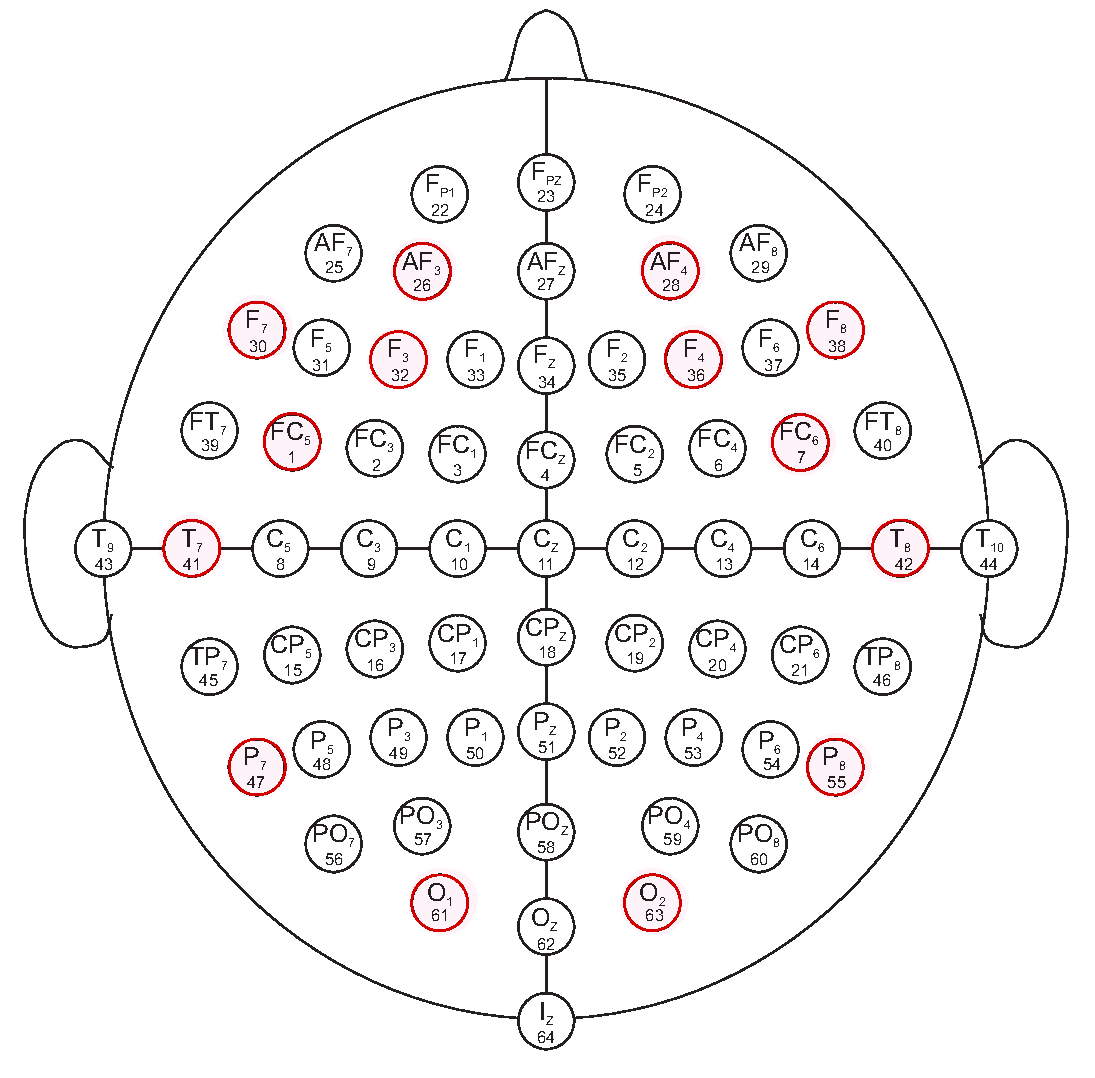
\includegraphics[width=0.45\textwidth]{64_channel_sharbrough.pdf}
\end{figure}
\end{frame}

%%%%%%%%%%%%%%%%%%%%%%%%%%%%%%%%%%%%%%%%%%%%%%%%%%%%%%%%%%%%%%%%%%%%%%%%%%%%%%%%%%%%%%%%%%%%%%%%%%%%%%%%%%%%%%%%%%%%%%%%%%%%%%%%%%%%%%%%%%%%%%%%%%%%%%%%%%%%%%%%%%%%%%%%%%%%%%%%%%%%%%%%%%%%%%%%%%%%%%%%%%%%%%%%%%%%
\begin{frame}{Данные для вычислительного эксперимента}
Основные характеристики выборки представлены в
Таблице~\ref{table:sample}.

\begin{table}
	\centering
	\caption{Описание выборки}
	\begin{tabular}{|c|c|c|}
		\hline
		Название                       & Обозначение & Значение             \\
		\hline \hline
		Продолжительность обследования & $\tau$         & 117 с                \\ \hline
		Частота измерения сигнала      & $\mu$       & 128.03 $\text{с}^{-1}$   \\ \hline
	    Число каналов (датчиков)    & $K$   & 14          \\ \hline
		Число измерений сигнала             & $T$  & 14980           \\ \hline
	\end{tabular}
	\label{table:sample}
\end{table}



\end{frame}
%%%%%%%%%%%%%%%%%%%%%%%%%%%%%%%%%%%%%%%%%%%%%%%%%%%%%%%%%%%%%%%%%%%%%%%%%%%%%%%%%%%%%%%%%%%%%%%%%%%%%%%%%%%%%%%%%%%%%%%%%%%%%%%%%%%%%%%%%%%%%%%%%%%%%%%%%%%%%%%%%%%%%%%%%%%%%%%%%%%%%%%%%%%%%%%%%%%%%%%%%%%%%%%%%%%%
\begin{frame}{Временные ряда в выборке}

\begin{figure}[h]
	\centering
	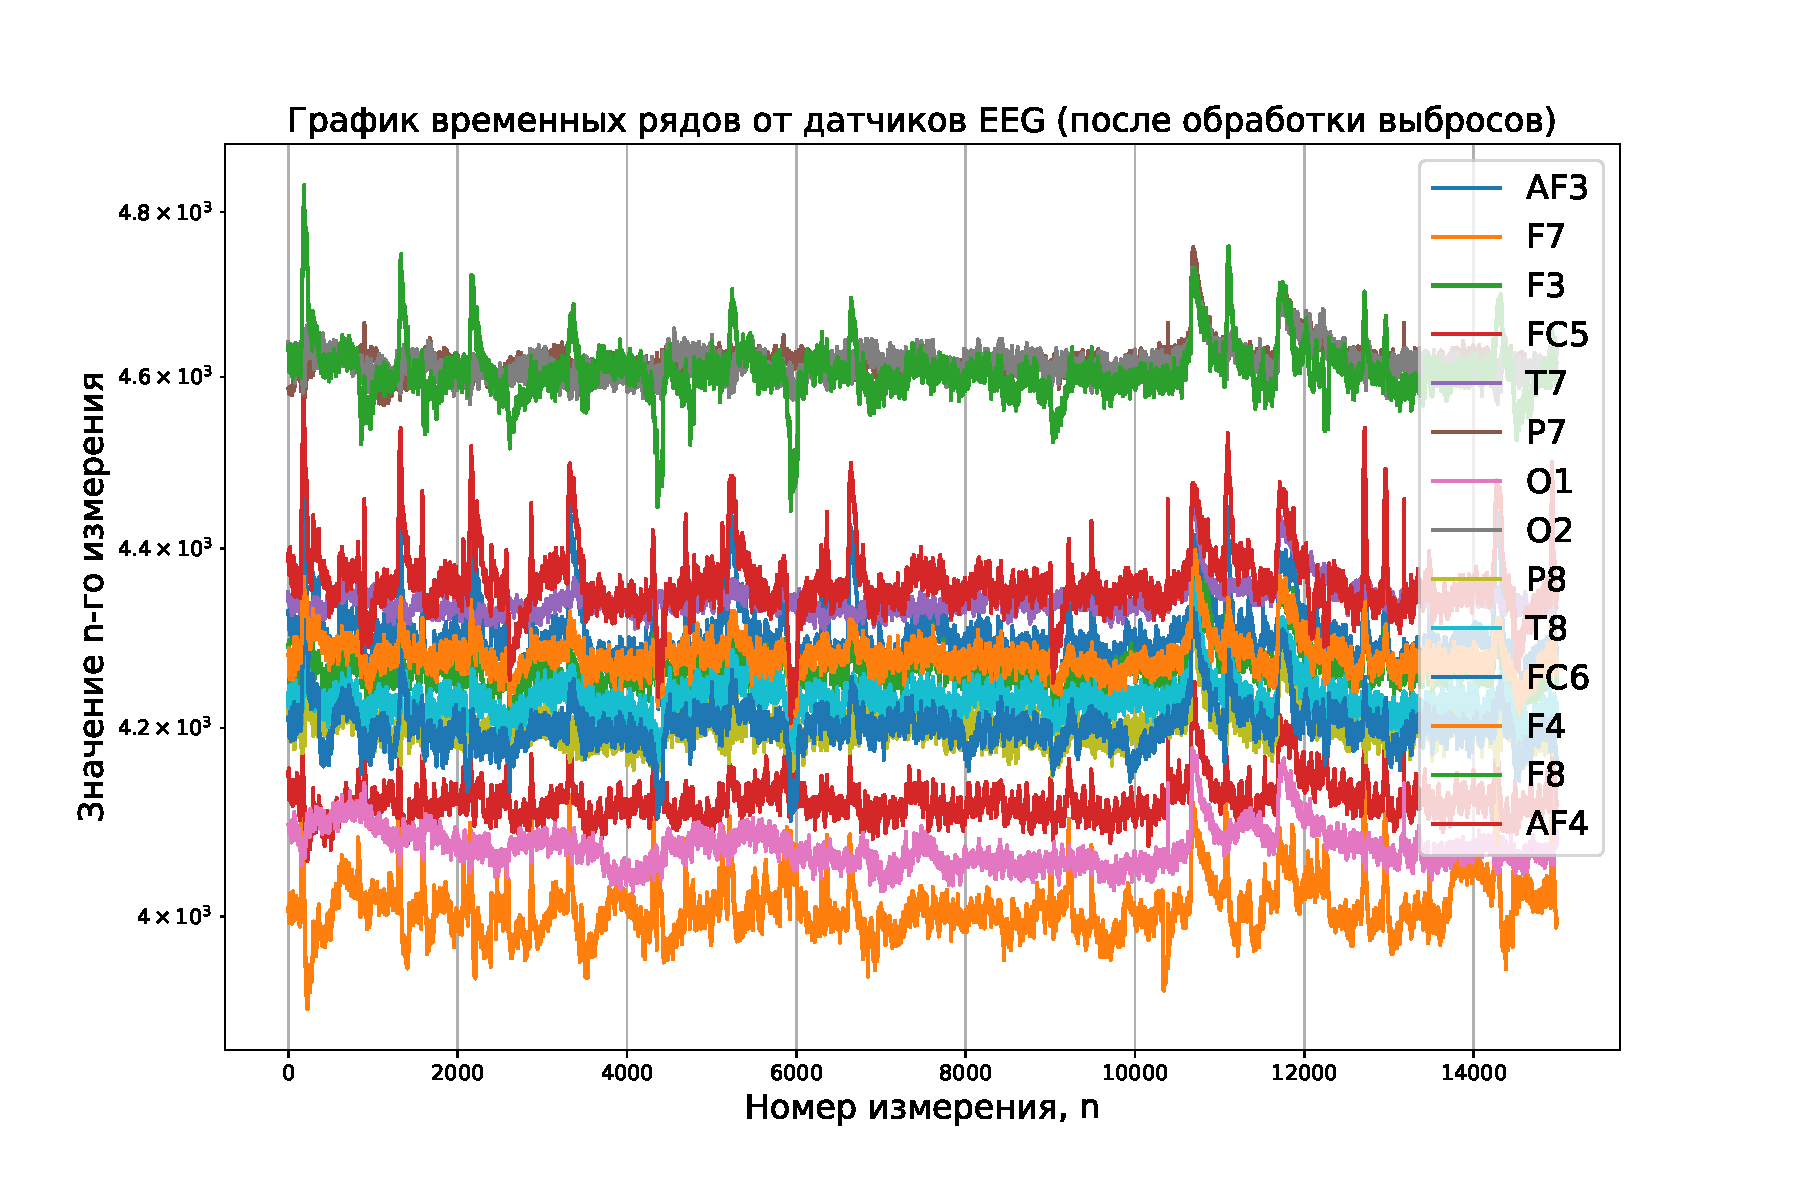
\includegraphics[width=0.8\textwidth]{Dataset.pdf}
	\caption{График временных рядов}
	\label{fig:2}
\end{figure}

\end{frame}
%%%%%%%%%%%%%%%%%%%%%%%%%%%%%%%%%%%%%%%%%%%%%%%%%%%%%%%%%%%%%%%%%%%%%%%%%%%%%%%%%%%%%%%%%%%%%%%%%%%%%%%%%%%%%%%%%%%%%%%%%%%%%%%%%%%%%%%%%%%%%%%%%%%%%%%%%%%%%%%%%%%%%%%%%%%%%%%%%%%%%%%%%%%%%%%%%%%%%%%%%%%%%%%%%%%%


\begin{frame}{Литература}
\nocite{barachant2010riemannian, misc_eeg_eye_state_264, congedo2013new}
\bibliographystyle{unsrt}
\bibliography{references}
\end{frame}
\end{document}